%%%%%%%%%%%%%%%%%%%%%%%%%%%%%%%%%%%%%%%%%%%%%%%%%%%%%%%%%%%%
% Paul McKee
% Rensselaer Polytechnic Institute
% 1/31/18
% Master's Thesis
% with Dr. Kurt Anderson
% LaTeX Template: Project Titlepage Modified (v 0.1) by rcx
%%%%%%%%%%%%%%%%%%%%%%%%%%%%%%%%%%%%%%%%%%%%%%%%%%%%%%%%%%%%

\documentclass[12pt]{report}
\iffalse
\usepackage[a4paper]{geometry}
\usepackage[utf8]{inputenc}
\usepackage[myheadings]{fullpage}
\usepackage{fancyhdr}
\usepackage{lastpage}
\usepackage{graphicx, wrapfig, subcaption, setspace, booktabs}
\usepackage[T1]{fontenc}
\usepackage[font=small, labelfont=bf]{caption}
\usepackage{fourier}
\usepackage[protrusion=true, expansion=true]{microtype}
\usepackage[english]{babel}
\usepackage{sectsty}
\usepackage{url, lipsum}
\usepackage{makecell}
\usepackage{amsmath}
\usepackage{setspace}
\usepackage{amsmath}
\usepackage{titlesec}
\usepackage[table,xcdraw]{xcolor}
%\titleformat{\section}{\normalfont\fontsize{25}{25}\bfseries}{\thesection}{1em}{}

%\usepackage[format=hang,font={small,bf},labelfont=bf]{caption}

\usepackage{listings}
\usepackage{color} %red, green, blue, yellow, cyan, magenta, black, white
\definecolor{mygreen}{RGB}{28,172,0} % color values Red, Green, Blue
\definecolor{mylilas}{RGB}{170,55,241}

%\newcommand{\HRule}[1]{\rule{\linewidth}{#1}}
\setcounter{tocdepth}{5}
\setcounter{secnumdepth}{5}
\usepackage{fancyhdr}
\usepackage{lastpage}
\usepackage{graphicx}
%\pagestyle{fancy}
%\fancyhf{Philip Hoddinott, Module 4 Questions}
\fancyhf{}
%\fancyhead[L]{Philip Hoddinott}
%\fancyhead[C]{Project 2}
%\fancyhead[R]{\leftmark}

\fancyhead[L]{Master's Thesis}
%\fancyhead[C]{\thepage}
%\fancyhead[R]{Module 5 Homework}
\fancyhead[C]{\leftmark}
\fancyhead[R]{Philip Hoddinott}
\fancypagestyle{plain}{
	\fancyfoot[C]{\thepage}}
\usepackage{float}

%\rfoot{Page \thepage \hspace{1pt} of \pageref{LastPage}}

\newcommand{\N}{\mathbb{N}}
\newcommand{\Z}{\mathbb{Z}}
\renewcommand{\headrulewidth}{0pt} % remove the header rule
\rfoot{\thepage}



\fi

\usepackage{graphicx, wrapfig, subcaption, setspace, booktabs}
\usepackage{sectsty}
\usepackage{url, lipsum}
\usepackage{makecell}
\usepackage{amsmath}
\usepackage{setspace}
\usepackage{amsmath}
\usepackage{color} %red, green, blue, yellow, cyan, magenta, black, white
\definecolor{mygreen}{RGB}{28,172,0} % color values Red, Green, Blue
\definecolor{mylilas}{RGB}{170,55,241}

\usepackage[table,xcdraw]{xcolor}


\usepackage[margin=1in]{geometry} 
\usepackage{amsmath,amsthm,amssymb}
\usepackage{color}
\usepackage{fancyhdr}
\usepackage{lastpage}
\usepackage{graphicx}

\pagestyle{fancy}
%\fancyhf{Philip Hoddinott, Module 5 Questions}
\fancyhf{}
%\fancyhead[L]{Philip Hoddinott}
%\fancyhead[C]{\thepage}
%\fancyhead[R]{Module 5 Questions}
\fancyhead[L]{Master's Thesis}
%\fancyhead[C]{\thepage}
%\fancyhead[R]{Module 5 Homework}
\fancyhead[C]{\leftmark}
\fancyhead[R]{Philip Hoddinott}

\rfoot{Page \thepage \hspace{1pt} of \pageref{LastPage}}

\newcommand{\N}{\mathbb{N}}
\newcommand{\Z}{\mathbb{Z}}

\newenvironment{theorem}[2][Theorem]{\begin{trivlist}
		\item[\hskip \labelsep {\bfseries #1}\hskip \labelsep {\bfseries #2.}]}{\end{trivlist}}
\newenvironment{lemma}[2][Lemma]{\begin{trivlist}
		\item[\hskip \labelsep {\bfseries #1}\hskip \labelsep {\bfseries #2.}]}{\end{trivlist}}
\newenvironment{exercise}[2][Exercise]{\begin{trivlist}
		\item[\hskip \labelsep {\bfseries #1}\hskip \labelsep {\bfseries #2.}]}{\end{trivlist}}
\newenvironment{problem}[2][Problem]{\begin{trivlist}
		\item[\hskip \labelsep {\bfseries #1}\hskip \labelsep {\bfseries #2.}]}{\end{trivlist}}
\newenvironment{question}[2][Question]{\begin{trivlist}
		\item[\hskip \labelsep {\bfseries #1}\hskip \labelsep {\bfseries #2.}]}{\end{trivlist}}
\newenvironment{corollary}[2][Corollary]{\begin{trivlist}
		\item[\hskip \labelsep {\bfseries #1}\hskip \labelsep {\bfseries #2.}]}{\end{trivlist}}

\newenvironment{solution}{\begin{proof}[Solution]}{\end{proof}}
\usepackage{multicol}
\newcommand{\mysize}{0.5}
\usepackage{subcaption}
\usepackage{float}
\usepackage{listings}
\usepackage{color} 
%\linespread{1.5}
\usepackage{setspace}



% %---------------------------------------------------------------
% % HEADER & FOOTER
% %---------------------------------------------------------------

%\fancyhf{}
%\pagestyle{fancy}
%\renewcommand{\headrulewidth}{0pt}
%\setlength\headheight{0pt}
%\fancyhead[L]{ Paul McKee }
%\fancyhead[R]{Rensselaer Polytechnic Institute}
%\cfoot{ \thepage\ } 


%--------------------------------------------------------------
% TITLE PAGE
%--------------------------------------------------------------

\begin{titlepage}
	\title{ 
		\LARGE \textbf{\uppercase{Tracking of space debris from publicly available data }} \\
		\vspace{0.25cm}
		\LARGE \textbf{Philip Hoddinott}
	}
	\author{\small{Submitted in Partial Fulfillment of the Requirements} \\ \small{for the Degree of} \\
		\uppercase{Master of Science} \\ \\
		Approved by:
		\\ Kurt Anderson, Chair \\ John Christian \\ Matthew Oehlschlaeger \\ \\ %% from paul's template
		
\includegraphics[width=2.5cm]{rensselaer_seal.png} \\
		\small{\textit{Department of Mechanical, Aerospace, and Nuclear Engineering}} \\
		\small{Rensselaer Polytechnic Institute} \\ 
		\small{Troy, New York} \\
		\small{November 2018}
	}
\end{titlepage}

\begin{document}
	\maketitle
	
	
	\pagenumbering{roman}
	\setcounter{page}{-1}
	% --Table of Contents----------
	\tableofcontents
	\newpage
	\newlength\longest
	\clearpage
	
	\thispagestyle{empty}
	\null\vfill
	
	\begin{figure}[!t]
		\begin{center}
			\settowidth\longest{\huge\itshape But, Captain, I cannot change;}
			\parbox{\longest}{%
				\raggedright{\huge\itshape%
					But, Captain, I cannot change the laws of physics\par\bigskip
				}   
				\raggedleft\Large{-Lt. Commander Scott (Scotty)}\par
				\raggedleft\Large{USS}\textit{ Enterprise}\par%
				
			}
		\end{center}
	\end{figure}
	
	\null\vfill
	%		\begin{figure}
	%	\centering
	%	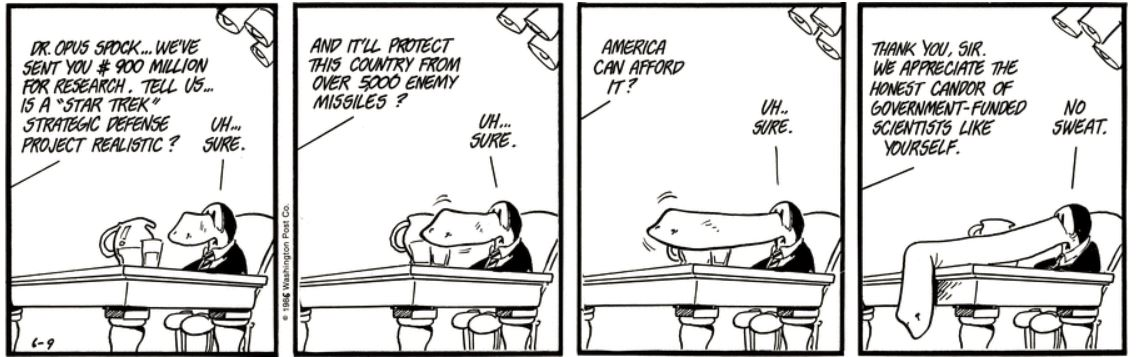
\includegraphics[width=0.7\linewidth]{../../Bloom_County_2}
	%	\caption*{}
	%	\label{fig:bloomcounty2}
	%\end{figure}
	
	\begin{figure}
		\centering
		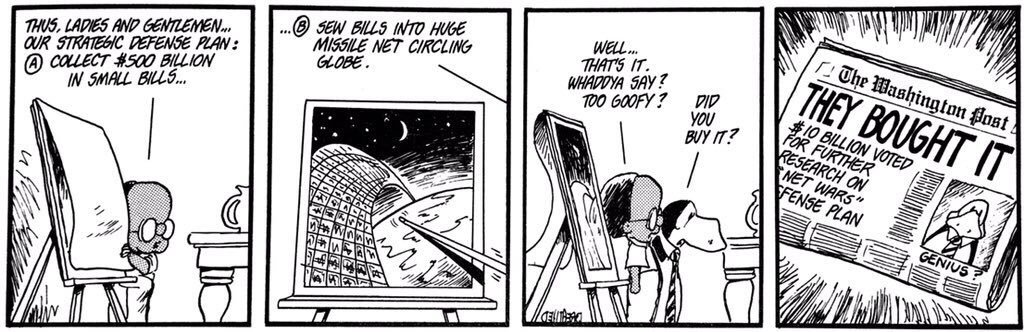
\includegraphics[width=0.7\linewidth]{../../Bloom_County}
		\caption*{}
		\label{fig:bloomcounty}
	\end{figure}
	
	\newpage

	%\thispagestyle{fancy}
	
	%\addcontentsline{toc}{section}{\uppercase{Table of Contents}}
	\listoftables
	%\addcontentsline{toc}{section}{\uppercase{List of Tables}}
	\listoffigures
	%\addcontentsline{toc}{section}{\uppercase{List of Figures}}
	% -----------------------------
	
	% ------------------------------------------------------------
	% Acknowledgement
	% ------------------------------------------------------------
	\newpage
		\doublespacing
	\section{Acknowledgments}
	%\addcontentsline{toc}{section}{\uppercase{Acknowledgement}}
	
	This paper would never have been possible with out the help of so many people. 
	I am indebted to my parents and my brother for their support. 
	
	John Benke for his assitance with Github and PHP. I am thankfull to Paul McKee for his assistance with Latex. 
	Thank lots of people here\par 
	
	Mom, dad, David,
	P Anderson
	John B for git and PHP
	Paul McKee for latex 
	
	
	
	

	
	% ------------------------------------------------------------
	% Abstract 
	% ------------------------------------------------------------
	
	\newpage
	\section{Abstract}
	The purpose of this project is to acquire information about earth orbiting debris, turn the information into a usable format, \textcolor{red}{and develop a targeting algorithm for a debris removal satellite}. The information is things such as orbital elements, debris size, \textcolor{red}{ and sping if i can find htis.} \par 
	 Should this be accomplished in a timely manner more work will be done on the orbital dynamics of OSCAR getting to said debris.
	% ------------------------------------------------------------
	% Introduction
	% ------------------------------------------------------------
	\newpage
	\pagenumbering{arabic} % this should start the normal numberinbg
	\section{Introduction}
	Before the methods of this project are explored, the background of the problem must first be presented. Space debris and the threat they pose will be explained, as well as the proposed solution. 
	

	\subsection{Space Debris}
	
	March 17th, 1958 the Vanguard 1 satellite was launched. It was the fourth man made satellite. Despite communication being lost in the 1960s, it is still in orbit to this day\cite{usnrl_2008}. \par 
	
	\begin{figure}[h!]
		\centering
		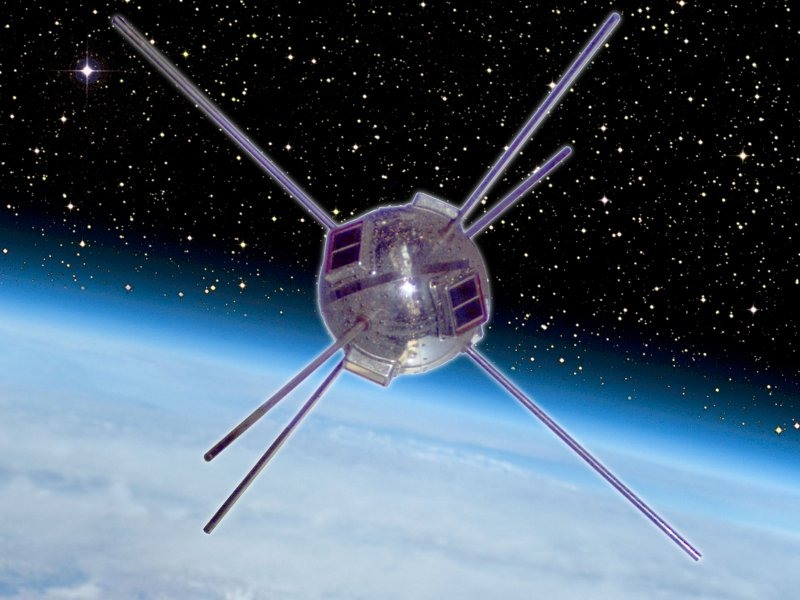
\includegraphics[width=0.7\linewidth]{Vanguard_1_composite}
		\caption{Artist's rendition of Vanguard 1 in orbit.}
		\label{fig:vanguard1composite}
	\end{figure}
	
	While spacecraft are supposed to be moved to a graveyard orbit, not all are. These large objects would be catastrophic if they collided with another object in orbit. However large objects do not pose the greatest threat. Their size makes them easy to track and there are comparatively little of them. 
	
	\begin{figure}
		\centering
		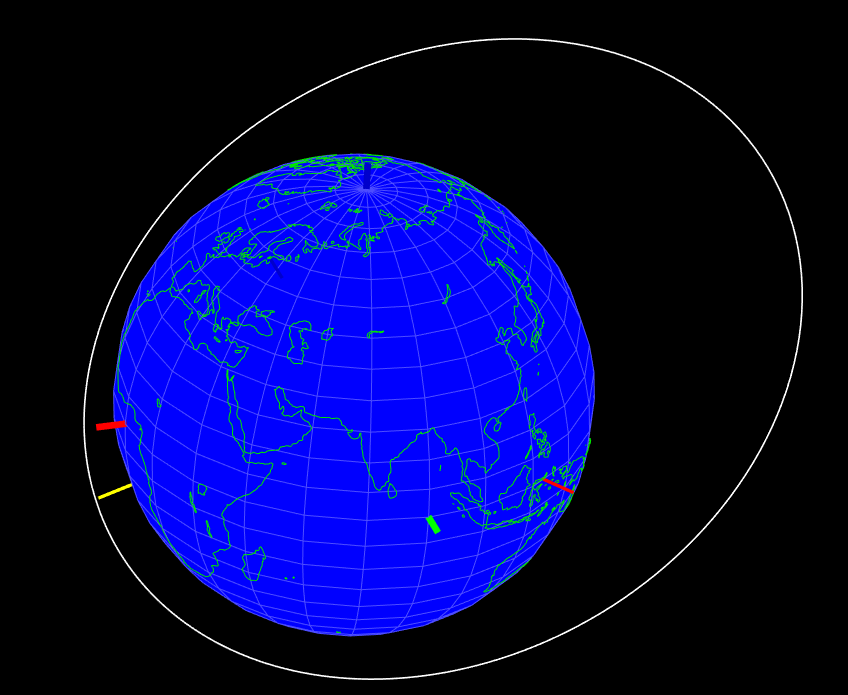
\includegraphics[width=0.7\linewidth]{Vanguard_1_orbit}
		\caption{Vanguard's Orbit as of 10/17/2018 \textcolor{red}{UPDATE THIS}}
		\label{fig:vanguard1orbit}
	\end{figure}

	The debris that poses the greatest threat are the smaller pieces. Their size makes them harder to track and predict trajectories. And they are numerous. As of 2013 it is estimated that there are:
	\newline
	\singlespacing
	29,000 Objects larger than 10 cm.\newline
	
	670,000 Objects larger than 1 cm.\newline
	
	Over 170,000,000 Objects larger than 1 mm.\newline 
	\doublespacing
	
	These objects can do grievous harm to people or objects in space. A 10 cm object can cause the destruction of a satellite, a 1 cm object could penetrate the ISS's shields putting lives at risk and a 1 mm object could destroy critical subsystems.\cite{sdor2014} The impact of one of these objects is shown in figure \ref{fig:sts7crack}.
	
	
	
	\begin{figure}
		\centering
		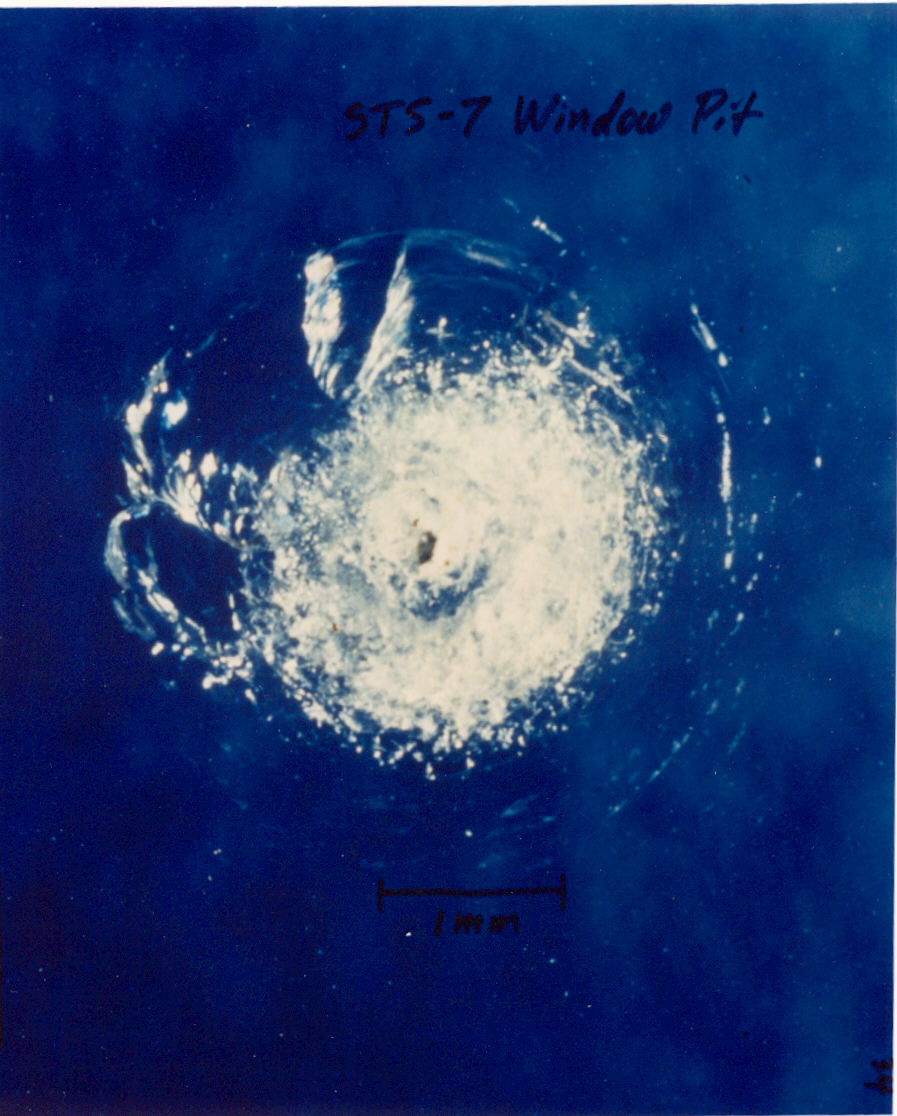
\includegraphics[width=0.7\linewidth]{sts7crack}
		\caption{An impact crater on one of the windows of the Space Shuttle Challenger following a collision with a micrometeoroid\cite{stscrack}}
		\label{fig:sts7crack}
	\end{figure}


\begin{figure}
	\centering
	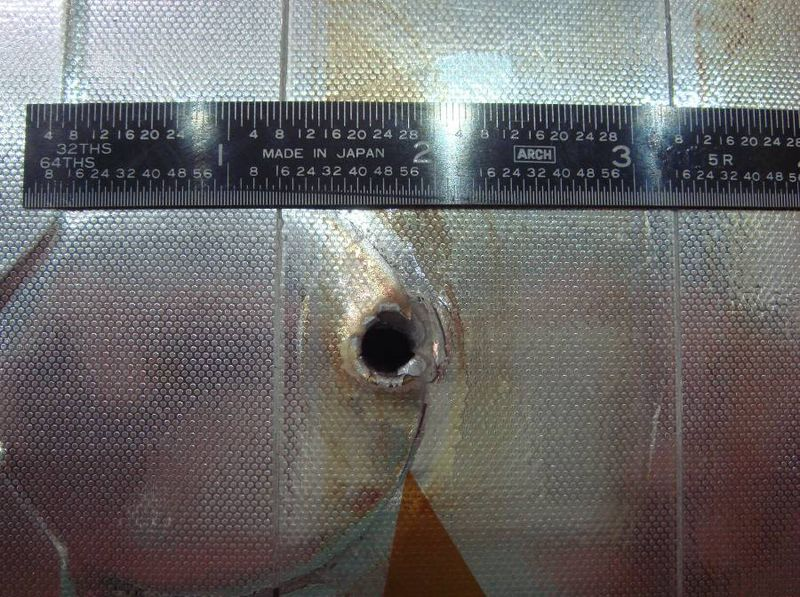
\includegraphics[width=0.7\linewidth]{STS-118_debris_entry}
	\caption{Debris impact on Space Shuttle Endeavorer's radiator panel\cite{endevHole}}
	\label{fig:sts-118debrisentry}
\end{figure}
	
	
	%\begin{align}
	%E=\frac{1}{2}mv^2
	%\end{align}
	%\begin{align}
	%E=\frac{1}{2}(.001kg)(7.66 \times 10^3)^2
	%\end{align}
	
	\subsection{Kessler Syndrome}
	More than just harm to individual spacecraft or persons there is the threat of Kessler Syndrome. Also known as the Kessler effect or collision cascading, this is a scenario where there are enough objects in low earth orbit that a collision between objects will cause a chain reaction creating more and more space debris. This could result in space being inaccessible for years to come, as any object that left the earth's atmosphere would be immediately shredded by debris (thus adding even more debris).\par 
	
	This can be prevented by moving derelict spacecraft to graveyard orbits. However even spacecraft in graveyard orbits are not perfectly safe. Coolant tanks can puncture and coolant droplets freeze adding to the debris. \par 
	
	The alternative is to lower the orbit until it experiences atmospheric effects. But if the debris's orbit keeps it out of the atmosphere, then the debris must be moved. 

	\subsection{CubeSats}
	For the task of moving debris, a CubeSat will be used. CubeSats are a type of miniaturized satellite. CubeSats get their name from their structure, they are made up of one or more $10\times10\times10$ cm units.	These units have a maximum mass of 1.33 kilograms. First launched in 1998, as of August 2018, there have been 875 CubeSats launched\cite{nanosats_eu}. \par 
	
	
	
	CubeSats are used for projects that are too risky for a larger more expensive satellite, often demonstrating new technologies. They can take on larger risks due to their low cost. As such CubeSats are common for experiential missions such as this one.
	
	\subsection{OSCAR}
	There is a CubeSat currently being designed by Rensselaer Polytechnic Institute (RPI). This CubeSat's goal is deorbit space debris by use of a magnetic tether. \par 
	
	
	This CubeSat is called O.S.C.A.R, which is short for “Obsolete Satellite Capture and Recovery”. It should be noted that this name is only temporary and will likely change in the near future. However for the purposes of this report, the RPI CubeSat will be referred to as OSCAR.\par 
	
	OSCAR will be a three unit  $(10\times10\times30)$ CubeSat with a mass of four kilograms. It will be able to remove four pieces of space debris.\cite{paulT}
	
	For OSCAR to be able to deorbit space debris, it must know where the space debris is. 
	
	\subsection{Orbital Elements}
	
	This thesis is concerned with the acquisition of current orbital data of space debris and it's transformation into useful formats. 
	
	First orbital elements should be defined. Orbital elements are the parameters that define an orbit. The traditional Keplerian elements found in many textbooks are as follows: 
	
	\begin{eqnarray}
	h& \text{specific angular momentum}\\
	i& \text{ inclination}\\
	\Omega &\text{ right ascension (RA) of the ascending node}\\
	e & \text{ eccentricity}\\
	\omega &\text{ argument of perigee}\\
	\theta &\text{ true anomaly}
	\end{eqnarray}
	
	However for the use of
	
	
	page 175
	
	Should I define Orbital Elements.

	
	% ------------------------------------------------------------
	% Spacecraft Dynamics
	% ------------------------------------------------------------
	\newpage
	\section{Data Sources and Formats}
	
	
	
	First data sources for space debris must be found, and the data formats must be understood. The most common data format for orbital elements is the Two Line Element Set (TLE). Despite the large number of objects in space, real time data is surprisingly hard to find. While there are various websites and programs to track the location of objects such as the International Space Station, debris from old spacecraft is not quite as popular. The website space-track.org publishes TLEs for public use. First the TLE format will be explained then their acquisition will be discussed. 
	
	
	
	
	\subsection{The Two Line Element Format}
	
	Orbital elements provide the means to determine a theoretical orbit. Since spacecraft are constantly experiencing forces such as atmospheric drag or solar wind their orbital elements are constantly changing. \par 
	A Two Line Element (TLE) is a data format that encodes a list of orbital elements for an Earth-orbiting object for a given point in time [\textcolor{red}{Re do this}]\par
	
	An example shows how orbital information is derived from a Two Line Element \cite{NASATLE}.
	\begin{figure}[h!]
		\centering
		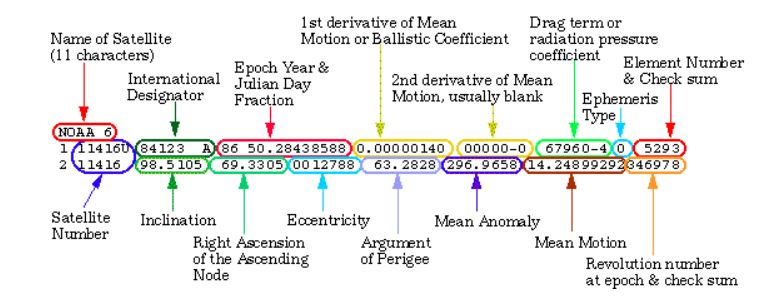
\includegraphics[width=0.7\linewidth]{tle_nasa}
		\caption{TLE with descriptions}
		\label{fig:tlenasa}
	\end{figure}
	
	\begin{enumerate}
		\item \textbf{Name of Satellite:} NOAA 6
		
		This is the name of the satellite. In this example it is NOAA 6.
		\item 	\textbf{International Designator:} 84123 A
		
		This number shows the last two digets of the launch year and what number launch of that year it was. In this example it is 84 123 A. The satellite was launched in the year 1984 and it was the 124th launch of the year. The A means that it was the first object that came from the launch. \textcolor{red}{Check this is right}
		
		\item \textbf{Epoch Date and Julian Date Fraction:} 86 50.28438588
		
		The Epoch date shows the year this TLE was made and the Julian Date fraction is the number of days in said year. 
		
		\item \textbf{First Derivative of Mean Motion:} 0.00000140
		
		This is the daily rate of change of number of revolutions the object completes per day divided by two. This is also called the ballistic coefficient.\cite{NASATLE} It's units are $\frac{rev}{day^2}$. 
		
		\item \textbf{Second Derivative of Mean Motion:} 00000-0
		
		This is the second derivative of mean motion divided by six, with units of $\frac{rev}{day^3}$.
		
		\item \textbf{Drag term or B* Term: }6970-4
		
		Of the terms given here, the B* term is the least heard of. It is a way of modeling drag on orbiting objects in propagation models.  
		Aerodynamic drag is given by the following equation:
		\begin{equation}
		F_D = \frac{1}{2}\rho C_d A v^2
		\end{equation}
		Where $A$ is the area, $C_d$ is the drag coefficient, $v$ the velocity, and $\rho$ is the fluid density. From Newton's second law
		\begin{equation}
		F = m\times a
		\end{equation}
		the accleration due to the force of drag is 
		\begin{equation}
		a_D=\frac{F_D}{m}=\frac{\rho C_d A v^2}{2m}=\frac{ C_d A}{m}\times\frac{\rho v^2}{2}
		\end{equation}
		The ballistic coefficient is given by the following equation:
		\begin{equation}
		B=\frac{ C_d A}{m}
		\end{equation}
		The starred ballistic coefficient is then
		\begin{equation}
		B^{*} = \frac{\rho_0 B}{2}=\frac{\rho_0 C_d A}{2m}
		\end{equation}
		This turns the equation for acceleration due to drag into \cite{celestrak_TLE_FAQ}\cite{castor2_BSTAR}
		\begin{equation}
		a_D=\frac{\rho}{\rho_0}B^{*} v^2
		\end{equation}
		\textcolor{red}{Possibly not needed maybe take out. }\par 
		\item \textbf{Element Set Number and Check Sum}
		
		\item \textbf{Satellite Number: } 11416U
		
		This is the Satellite Catalog Number and designation of the object. A U means unclassified. 
		
		\item \textbf{Inclination (degrees): }98.5105
		
		This is one of the orbital elements.
		\item \textbf{Right Ascension of the Ascending Node (degrees): }69.3305
		
		This is one of the orbital elements.
		
		\item \textbf{Eccentricity: } 0012788
		
		This is one of the orbital elements.
		
		\item \textbf{Argument of Perigee (degrees): }63.2828
		
		This is one of the orbital elements.
		
		\item \textbf{Mean Anomaly (degrees): }296.9658
		
		This is one of the orbital elements.
		
		\item \textbf{Mean Motion: } 14.24899292
		
		This is the orbits per day the object completes. 
		
		\item \textbf{Revolution Number and Check Sum: } 346978
		
		
		
		
	\end{enumerate}

\par 
	
\newpage	
	\singlespacing
A second example is given below. This time with references to the position of values, for extraction. The line under the dashes is the reference number line.
	\begin{verbatim}
	ISS (ZARYA)
	1 25544U 98067A   04236.56031392  .00020137  00000-0  16538-3 0  9993
	2 25544  51.6335 344.7760 0007976 126.2523 325.9359 15.70406856328906
	----------------------------------------------------------------------
	1234567890123456789012345678901234567890123456789012345678901234567890   
	1         2         3         4         5         6         7
	
	\end{verbatim}
	Table \ref{tab:TLE_Desc} describes the second example TLE\cite{SpaceTrackTLE}. 
	% Please add the following required packages to your document preamble:
	% \usepackage{graphicx}
	% \usepackage[table,xcdraw]{xcolor}
	% If you use beamer only pass "xcolor=table" option, i.e. \documentclass[xcolor=table]{beamer}
	
	% Please add the following required packages to your document preamble:
	% \usepackage{graphicx}
	% \usepackage[table,xcdraw]{xcolor}
	% If you use beamer only pass "xcolor=table" option, i.e. \documentclass[xcolor=table]{beamer}
		\begin{table}[h!]
		\centering
		\caption{Description of TLE}
		\label{tab:TLE_Desc}
		\resizebox{\textwidth}{!}{%
			\begin{tabular}{|l|l|l|}
				\hline
				\multicolumn{3}{|l|}{\textbf{Line 0}}                                                                                                                               \\ \hline
				\rowcolor[HTML]{333333} 
				{\color[HTML]{FFFFFF} \textbf{Columns}} & {\color[HTML]{FFFFFF} \textbf{Example}} & {\color[HTML]{FFFFFF} \textbf{Description}}                                     \\ \hline
				1-24                                    & ISS (ZARYA)                             & The common name for the object based on information from the Satellite Catalog. \\ \hline
				\multicolumn{3}{|l|}{\textbf{Line 1}}                                                                                                                               \\ \hline
				\rowcolor[HTML]{333333} 
				{\color[HTML]{FFFFFF} \textbf{Columns}} & {\color[HTML]{FFFFFF} \textbf{Example}} & {\color[HTML]{FFFFFF} \textbf{Description}}                                     \\ \hline
				1                                       & 1                                       & Line Number                                                                     \\ \hline
				3-7                                     & 25544                                   & Satellite Catalog Number                                                        \\ \hline
				8                                       & U                                       & Elset Classification                                                            \\ \hline
				10-11                                   & 98                                      & International Designator (Last two digits of launch year)                       \\ \hline
				12-14                                   & 067                                     & International Designator (Launch number of the year)                            \\ \hline
				15-17                                   & A                                       & International Designator (Piece of the launch)                                  \\ \hline
				19-32                                   & 04                                      & Epoch Year (last two digits of year)                                            \\ \hline
				21-32                                   & 236.56031392                            & Epoch (day of the year and fractional portion of the day)                       \\ \hline
				34-43                                   & .00020137                               & 1st Derivative of the Mean Motion with respect to Time                          \\ \hline
				45-52                                   & 00000-0                                 & 2nd Derivative of the Mean Motion with respect to Time (decimal point assumed)  \\ \hline
				54-61                                   & 16538-3                                 & B* Drag Term                                                                    \\ \hline
				63                                      & 0                                       & Element Set Type                                                                \\ \hline
				65-68                                   & 999                                     & Element Number                                                                  \\ \hline
				69                                      & 3                                       & Checksum                                                                        \\ \hline
				\multicolumn{3}{|l|}{\textbf{Line 2}}                                                                                                                               \\ \hline
				\rowcolor[HTML]{333333} 
				{\color[HTML]{FFFFFF} \textbf{Columns}} & {\color[HTML]{FFFFFF} \textbf{Example}} & {\color[HTML]{FFFFFF} \textbf{Description}}                                     \\ \hline
				1                                       & 2                                       & Line Number                                                                     \\ \hline
				3-7                                     & 25544                                   & Satellite Catalog Number                                                        \\ \hline
				9-16                                    & 51.6335                                 & Orbit Inclination (degrees)                                                     \\ \hline
				18-25                                   & 344.7760                                & Right Ascension of Ascending Node (degrees)                                     \\ \hline
				27-33                                   & 0007976                                 & Eccentricity (decimal point assumed)                                            \\ \hline
				35-42                                   & 126.2523                                & Argument of Perigee (degrees)                                                   \\ \hline
				44-51                                   & 325.9359                                & Mean Anomaly (degrees)                                                          \\ \hline
				53-63                                   & 15.70406856                             & Mean Motion (revolutions/day)                                                   \\ \hline
				64-68                                   & 32890                                   & Revolution Number at Epoch                                                      \\ \hline
				69                                      & 6                                       & Checksum                                                                        \\ \hline
			\end{tabular}%
		}
	\end{table}
	
	

	\textcolor{red}{to do here, add more details on what the checksum and stuff like that is}
	
	\par 
		\doublespacing
	The process of TLE gathering and updating is somewhat shadowy. \cite{vallado2012two} What is known is that observations are collected multiple times per day at the Joint
	Space Operations Center (JSPOC) which is operated by the US Air Force Space Command (AFSPC). Then the unclassified TLEs are passed on to space-track for public release.  
	
	\subsection{Space-Track.org}
	Information about objects in space may be found the website space-track.org. Space-track is the main source for orbital data, though some are also available from the website celestrak.com. Of the two space-track has far more information and better methods of access.  "Space-Track.org is managed, maintained and administered by JFSCC"\cite{SpaceTrackLegend}.   \textcolor{red}{Put more information about the website here}.\par 
	space-track allows information to be downloaded manually from the TLE search \cite{SpaceTrackTLE} or the satellite catalog search \cite{SpaceTrackSATCAT}. While these are useful tools the code needs a way to automatically download data. Fortunately space-track also has an API that allows queries. 
	\subsection{Space-Track Query}
	\subsection{SatCat?}
	\section{NORAD Space-Track}	
	Describe the site
	desribe the SATCAT, then the TLE query
	
	
	
	
	\section{Code Overview}
	The code obtains orbital data for space debris depending on what variables the user has inputted, such as the launch year of the debris or how recent the data should be.
	First the code ascertains what data is already available. It checks to see if there is a .mat file for the SATCAT. This is simply a file that contains the catalog ids of the debris. If this file does not exist then the code has not been run for the current parameters, and the code will be run. \par 
	The code will also check to see if there is a TLE .mat file. If this file exists the code then checks when the file was created. Depending on user variables, the code may consider the information to be out of date, will rerun everything. However if the TLE .mat file is recent, then the code will load the current debris data into the workspace.\par 
	Assuming that the code detects that it has no data, or the data is out of date the code will work in the following steps\par 
	\begin{enumerate}
		\item The desired NORAD satellite catalog ids will be collected with the get\_SATCAT.m file. These ids are determined by user variables such as launch date. The code downloads them as a csv, strips things like quotation marks away, and sorts the ids in order.
		\begin{itemize}
			\item if a SATCAT .mat file exists and is recent this step is skipped.
		\end{itemize}  
		\item The code then downloads the TLEs as .txt files from the satellite ids. It does this in groups that have their size determined by the user. 
		\item The .txt files are then parsed, the TLEs are turned into usable orbital information, and saved as an array in MATLAB. This is done in the readTLE\_txt.m file.
		\item Finally the array of debris information is sorted in order of satellite id and duplicate rows are removed. It should be noted that not all TLEs requested will be provided. So if the code requests TLEs of objects with a id from 1000 to 1100 and expects 100 TLEs, but some are classified, then duplicated TLEs will be returned to make 100 TLEs. As such these duplicates must be removed. The final array is stored in a .mat file with it's date of creation noted. The user now has a usable list of space debris and their orbital elements.
	\end{enumerate}

	What now follows is a more in depth explanation of each file. 
		\subsection{VarStore.m}
		This is a file where a few imporant variables are stored. Depening on how the code is reformatted, it might get deleted.\textcolor{red}{COME BACK TO THIS}
		\subsection{UserPass.m}at
		This file is where the username and password for space-track.org are stored. 
		\subsection{MASTER\_TLE.m}
		This file is the master file for the Two Line Element MATLAB files. Running it will run all of the associated MATLAB files. These MATLAB files take some time to run, so it may be convenient to toggle the files run by the MASTER\_TLE.m
		\subsection{get\_SATCAT.m}
		Get\_SATCAT.m is the MATLAB file that gets the satellite catalog  numbers of all orbital debris launched after a given year and with the “RCS\_SIZE” value equal to “SMALL”. The Launch Year can be set by the values given by the user in VarStore.m The default launch year is set to 1990. Note that an earlier launch year will provide more data, and thus it will take more time to process. This may cause a time out error. Should this happen the timeOutVal in VarStore.m should be adjusted to be longer.\par 
		Once the SATCAT csv file has been acquired the file then formats it. The quotation marks that are around every entry are removed. The debris that have already deorbited are also removed. Finally the debris is sorted by NORAD Catoluge Id, and saved as a .mat file.
		\subsection{get\_Multiple\_TLE\_from\_Id.m}
		This file takes the Ids given in the .mat file and then obtains the Two Line Element files associated with the debris. It does this by saving the TLEs in .txt files. The number of TLEs grabbed at a time and saved in a .txt file is set by the user. It is not advised to go above 400, as that causes time out errors. \par 
		Withing MASTER\_TLE.m, this code is surrounded by a a loop and a try/catch error. The loop runs through all the different blocks of TLEs. In the case of a time out the the try/catch will attempt to download the TLEs a second time.\par 
		At this point in the code the space debris has had it's Two Line Element files saved to .txt files. This is the longest part of the code to run, but also with the .txt files saved, these functions need only be run once every few days. 

		\subsection{readTLE\_txt.m}
		This MATLAB file reads the .txt files and then converts the TLE format to the standard orbital elements stored in a .mat file. 
		%\subsection{check\_TLE\_Edit\_TLE.m}
		
		
		\section{Targeting}
		Once the data has been collected, the next step is to target possible orbits. Since OSCAR has a delta V of \textcolor{red}{Find delta V} inclanation and plane changes are out of the question. What is desired is a number of debris in a plane with simialr inclanations.
		
		\begin{figure}[!]
			\centering
			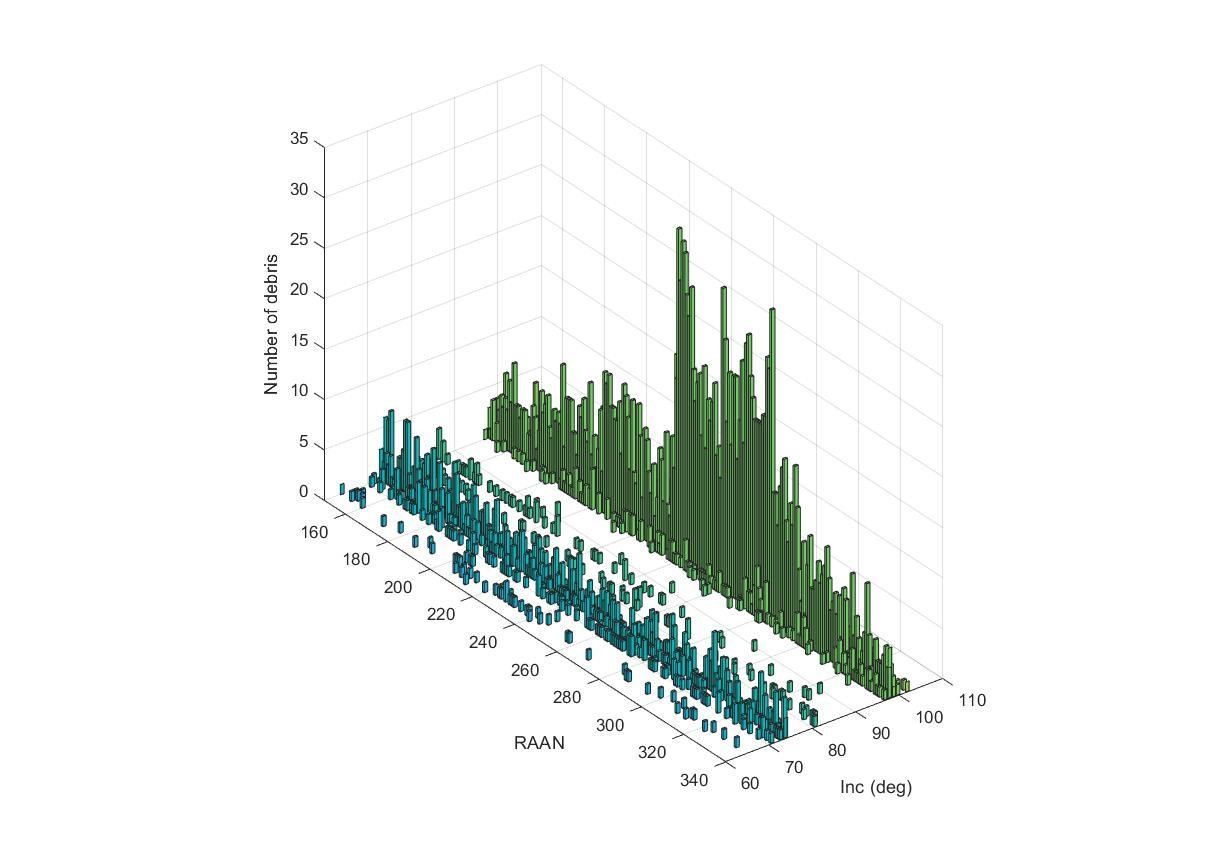
\includegraphics[width=0.7\linewidth]{rann_inc}
			\caption{Debis loc}
			\label{fig:ranninc}
		\end{figure}
		
	
	\section{Conclusion}
	The goal of this thesis was to create a program that can download the latest orbital elements needed to calculate the real time locations of space debris, given user inputted parameters. The information would be usable to someone who has taken a basic spaceflight mechanics class. 
	

	
		
		%--------------------------------------
		% References
		% -------------------------------------
		
		\bibliographystyle{unsrt}
		\bibliography{ref}

		
		%-----------------------------------------------------------
		% Appendix
		%-----------------------------------------------------------
		\newpage
		\section*{Appendix 1 - MATLAB code}
		\addcontentsline{toc}{section}{Appendix}
		
		\lstset{language=Matlab,%
			%basicstyle=\color{red},
			breaklines=true,%
			morekeywords={matlab2tikz},
			keywordstyle=\color{blue},%
			morekeywords=[2]{1}, keywordstyle=[2]{\color{black}},
			identifierstyle=\color{black},%
			stringstyle=\color{mylilas},
			commentstyle=\color{mygreen},%
			showstringspaces=false,%without this there will be a symbol in the places where there is a space
			numbers=left,%
			numberstyle={\tiny \color{black}},% size of the numbers
			numbersep=9pt, % this defines how far the numbers are from the text
			emph=[1]{for,end,break},emphstyle=[1]\color{red}, %some words to emphasise
			%emph=[2]{word1,word2}, emphstyle=[2]{style},    
		}
		
	%Thanks for Paul McKee who started this template. It seems to have good matlab code viwing
		
	\end{document}
	
